% 16:9 is a beamer class option, so the moloch docs never mention it
\documentclass[aspectratio=169]{beamer}
\usetheme{moloch}

\usepackage{fontspec}
\setsansfont{Fira Sans}[BoldFont={Fira Sans SemiBold}]
\setmonofont{Fira Mono}

\usepackage{booktabs}
\usepackage{appendixnumberbeamer}
\graphicspath{{../thud/images/}}

% accent taken from the thesis (bindingcolor)
\definecolor{accent}{RGB}{0,90,156}
\molochcolors{
  progressbar fg=accent,
  alerted text=accent,
  frametitle bg=accent,
}

\title{Detecting Routing Failures in LLM-based Multi-Agent Systems through Linear Probes}
\subtitle{Master's thesis defence}
\author{Andrea Cantarutti}
\institute{Università degli Studi di Udine \\ Supervisor: Prof.\ Giorgio Brajnik \quad Co-supervisor: Prof.\ Kevin Roitero}
\date{}

\begin{document}

\maketitle

\begin{frame}{Outline}
  \tableofcontents
\end{frame}

\section{Problem}

\begin{frame}{Coordinators route requests to experts}
  \begin{columns}[T]
    \column{0.45\textwidth}
      \begin{itemize}
        \item a coordinator reads a developer request
        \item it picks one sub-agent (expert) to handle it
        \item a wrong pick is a \alert{routing failure}
      \end{itemize}
    \column{0.5\textwidth}
      \centering
      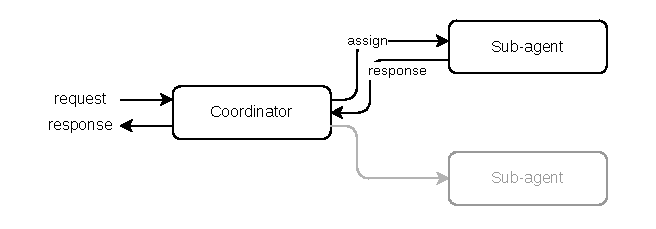
\includegraphics[width=\linewidth]{routing_response_coordinator.pdf}
  \end{columns}
\end{frame}

\begin{frame}{Five experts, one binding constraint}
  \centering
  \begin{tabular}{ll}
    \toprule
    Expert & Optimises for \\
    \midrule
    \texttt{time\_to\_market} & shipping fast \\
    \texttt{scale\_arch} & growth in load \\
    \texttt{resource\_opt} & cost and resources \\
    \texttt{legacy\_compat} & existing systems \\
    \texttt{strict\_compliance} & regulation \\
    \bottomrule
  \end{tabular}
\end{frame}

\section{Method}

\begin{frame}{Dataset generation}
  \centering
  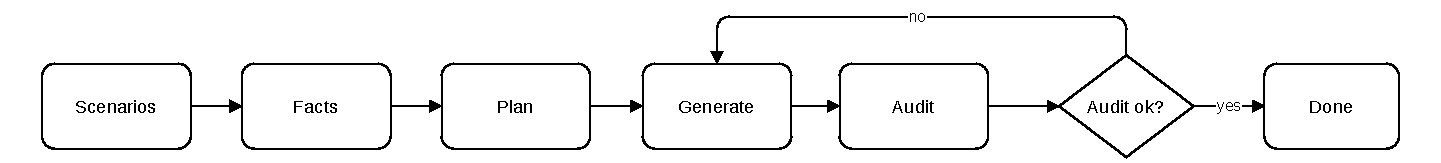
\includegraphics[width=0.9\textwidth,height=0.7\textheight,keepaspectratio]{generation_pipeline.pdf}
\end{frame}

\begin{frame}{Probing the hidden states}
  \begin{block}{Research question}
    Does a hidden layer encode the right expert more accurately than the model's own choice?
  \end{block}
  \begin{alertblock}{Requirement}
    The label must not be readable from the request text alone.
  \end{alertblock}
  \begin{exampleblock}{Approach}
    One linear probe per layer, compared against text-only baselines.
  \end{exampleblock}
\end{frame}

\section{Results}

\begin{frame}{Probe accuracy per layer}
  \centering
  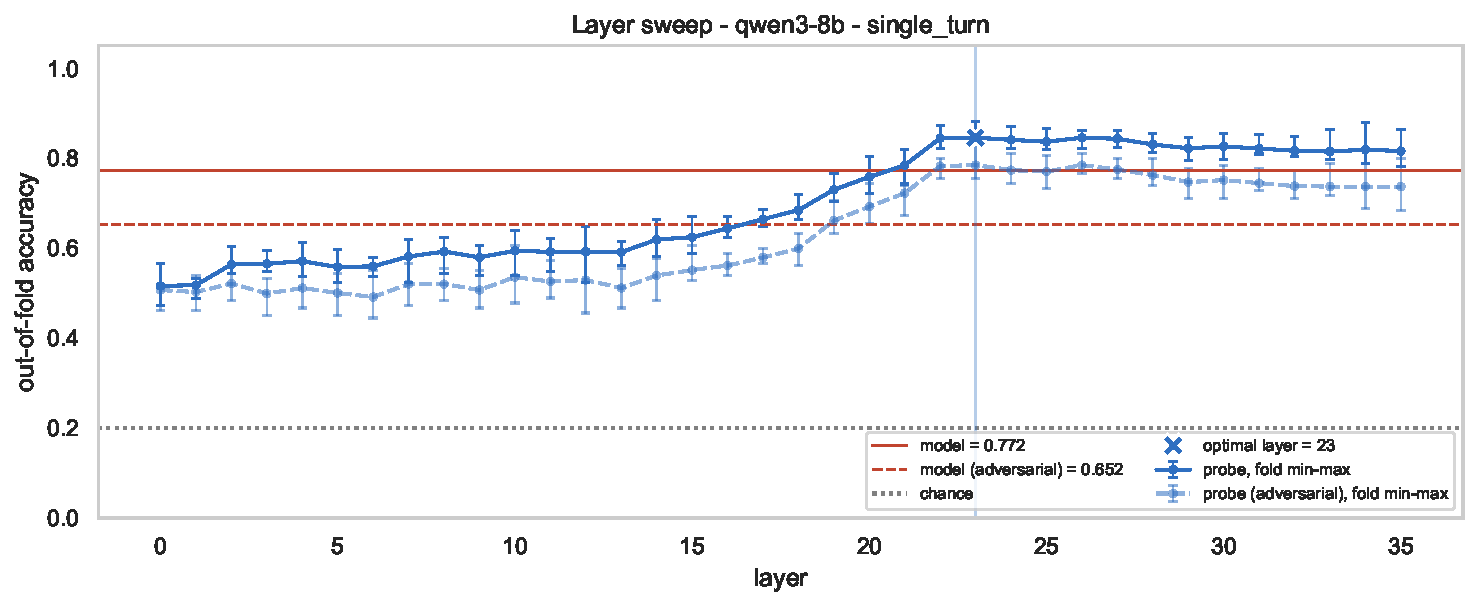
\includegraphics[width=\textwidth,height=0.75\textheight,keepaspectratio]{models/qwen3-8b_single_turn_layers.pdf}
\end{frame}

\begin{frame}[standout]
  Example standout slide \\[0.5em]
  for the one-line takeaway
\end{frame}

\begin{frame}{Conclusions}
  \begin{enumerate}
    \item first conclusion
    \item second conclusion
    \item future work
  \end{enumerate}
\end{frame}

\appendix

\begin{frame}{Backup: router comparison}
  \centering
  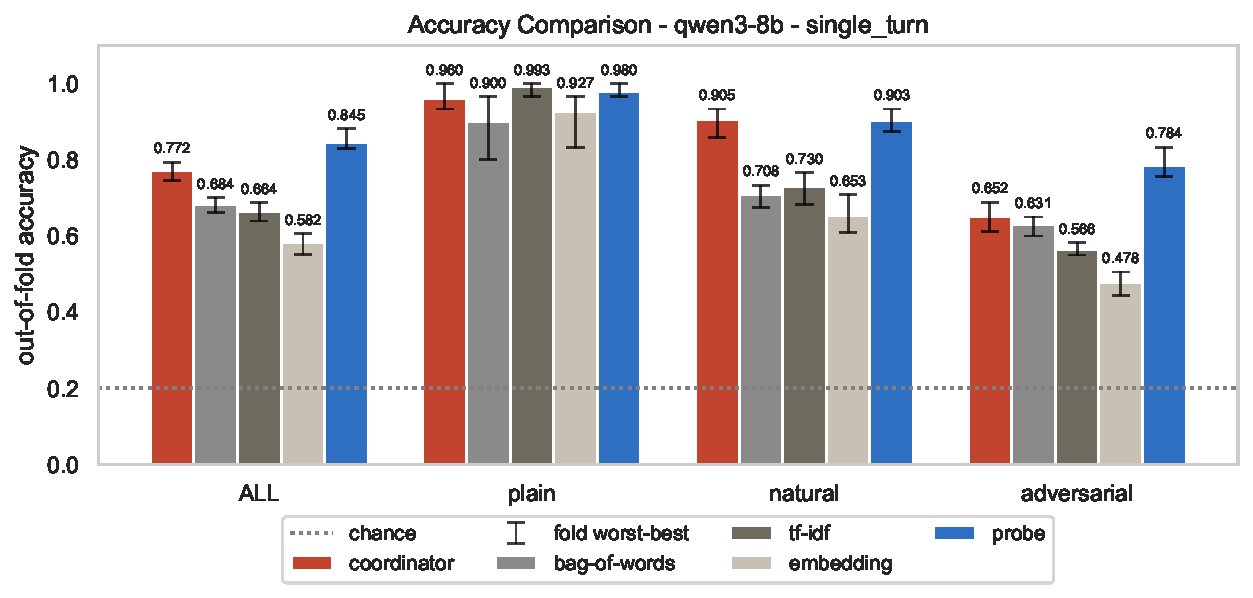
\includegraphics[width=\textwidth,height=0.75\textheight,keepaspectratio]{models/qwen3-8b_single_turn_routers.pdf}
\end{frame}

\end{document}
